%  LaTeX support: latex@mdpi.com
%  In case you need support, please attach any log files that you could have, and specify the details of your LaTeX setup (which operating system and LaTeX version / tools you are using).

%=================================================================

% LaTeX Class File and Rendering Mode (choose one)
% You will need to save the "mdpi.cls" and "mdpi.bst" files into the same folder as this template file.

%=================================================================

\documentclass[atoms,article,submit,moreauthors,pdftex,12pt,a4paper]{mdpi} 
%--------------------
% Class Options:
%--------------------
% journal
%----------
% Choose between the following MDPI journals:
% actuators, administrativesciences, aerospace, agriculture, agronomy, algorithms, animals, antibiotics, antibodies, antioxidants, appliedsciences, arts, atmosphere, atoms, axioms, batteries, behavioralsciences, bioengineering, biology, biomedicines, biomolecules, biosensors, brainsciences, buildings, cancers, catalysts, cells, challenges, chemosensors, children, chromatography, climate, coatings, computation, computers, cosmetics, crystals, dentistryjournal, diagnostics, diseases, diversity, econometrics, economies, education, electronics, energies, entropy, environmentalsciences, environments, epigenomes, fibers, foods, forests, futureinternet, gvalaxies, games, gels, genealogy, genes, geosciences, healthcare, horticulturae, humanities, hydrology, informatics, information, inorganics, insects, ijerph, ijfs, ijms, ijgi, jcdd, jcm, jdb, jfb, jimaging, jof, joi, jlpea, jmse, jpm, jrfm, jsan, land, laws, life, lubricants, machines, marinedrugs, materials, mathematics, medicalsciences, membranes, metabolites, metals, microarrays, micromachines, microorganisms, minerals, molbank, molecules, nanomaterials, ncrna, nutrients, pathogens, pharmaceuticals, pharmaceutics, pharmacy, photonics, plants, polymers, processes, proteomes, publications, religions, remotesensing, resources, risks, robotics, safety, sensors, sinusitis, socialsciences, societies, sports, standards, sustainability, symmetry, systems, technologies, toxics, toxins, universe, vaccines, veterinarysciences, viruses, water
%---------
% article
%---------
% The default type of manuscript is article, but could be replaced by using one of the class options: 
% article, review, communication, commentary, bookreview, correction, addendum, editorial, changes, supfile, casereport, comment, conceptpaper, conferencereport, meetingreport, discussion, essay, letter, newbookreceived, opinion, projectreport, reply, retraction, shortnote, technicalnote, creative
%----------
% submit
%----------
% The class option "submit" will be changed to "accept" by the Editorial Office when the paper is accepted. This will only make changes to the frontpage (e.g. the logo of the journal will get visible), the headings, and the copyright information. Journal info and pagination for accepted papers will also be assigned by the Editorial Office.
% Please insert a blank line is before and after all equation and eqnarray environments to ensure proper line numbering when option submit is chosen
%------------------
% moreauthors
%------------------
% If there is only one author the class option oneauthor should be used. Otherwise use the class option moreauthors.
%---------
% pdftex
%---------
% The option "pdftex" is for use with pdfLaTeX only. If eps figure are used, use the optioin "dvipdfm", with LaTeX and dvi2pdf only.

%=================================================================
\setcounter{page}{1}
\lastpage{x}
\doinum{10.3390/------}
\pubvolume{xx}
\pubyear{2015}
%\externaleditor{Academic Editor: xx}
\history{Received: xx / Accepted: xx / Published: xx}
%------------------------------------------------------------------
% The following line should be uncommented if the LaTeX file is uploaded to arXiv.org
%\pdfoutput=1

%=================================================================

% Add packages and commands to include here
% The amsmath, amsthm, amssymb, hyperref, caption, float and color packages are loaded by the MDPI class.
\usepackage{graphicx}
\usepackage{color}
\usepackage{verbatim}
%\usepackage{subfigure,psfig}

%=================================================================
%% Please use the following mathematics environments:
%\theoremstyle{mdpi}
%\newcounter{thm}
%\setcounter{thm}{0}
%\newcounter{ex}
%\setcounter{ex}{0}
%\newcounter{re}
%\setcounter{re}{0}
%\newtheorem{Theorem}[thm]{Theorem}
%\newtheorem{Lemma}[thm]{Lemma}
%\newtheorem{Characterization}[thm]{Characterization}
%\newtheorem{Proposition}[thm]{Proposition}
%\newtheorem{Property}[thm]{Property}
%\newtheorem{Problem}[thm]{Problem}
%\newtheorem{Example}[ex]{Example}
%\newtheorem{Remark}[re]{Remark}
%\newtheorem{Corollary}[thm]{Corollary}
%\newtheorem{Definition}[thm]{Definition}
%% For proofs, please use the proof environment (the amsthm package is loaded by the MDPI class).

%=================================================================
\def\be{\begin{equation}}
\def\ee{\end{equation}}
\def\ba{\begin{eqnarray}}
\def\ea{\end{eqnarray}}
% Full title of the paper (Capitalized)
\Title{Cavity-Assisted Spin-Orbit Coupling of Ultracold atoms}

% Authors (Add full first names)
\Author{Lin Dong $^{1,}$, Chuanzhou Zhu $^{1}$ and Han Pu $^{1}$*}

% Affiliations / Addresses (Add [1] after \address if there is only one affiliation.)
\address{%
$^{1}$ Department of Physics and Astronomy, Rice Quantum Institute, Rice University, Houston, Texas, 77251-1892, USA
}


% Contact information of the corresponding author (Add [2] after \corres if there are more than one corresponding author.)
\corres{hpu@rice.edu}

% Abstract (Do not use inserted blank lines, i.e. \\) 
\abstract{We investigate dynamical and static properties of ultracold atoms confined in an optical cavity, where two photon Raman process induces effective coupling between atom's internal degrees of freedom and center-of-mass motion. In the meantime, atomic dynamics exerts a back action to cavity photons. We adopt both mean field and master equation approach to tackle the problem and found surprising modifications to atomic dispersions and dynamical instabilities, arising from the intrinsic nonlinearity of the system. Correspondence between semi-classical and quantum limits is analyzed as well.}

% Keywords: add 3 to 10 keywords
\keyword{cavity quantum electrodynamics; cold atoms; spin-orbit coupling}

% The fields PACS, MSC, and JEL may be left empty or commented out if not applicable
%\PACS{}
%\MSC{}
%\JEL{}

% If this is an expanded version of a conference paper, please cite it here: enter the full citation of your conference paper, and add $^\dagger$ in the end of the title of this article.
%\conference{}

\begin{document}

%%%%%%%%%%%%%%%%%%%%%%%%%%%%%%%%%%%%%%%%%%

\section{Introduction}
%%%%%%%%%%%%%%%%%%%%%%%%%%%%%%%%%%%%%%%%%%
%\subsection{This is a Subsection Heading}
%%%%%%%%%%%%%%%%%%%%%%%%%%%%%%%%%%%%%%%%%%

When Jaynes and Cummings first studied the time evolution of a two-level atom in an electromagnetic field in a {\em fully} quantized way in 1960s \cite{JCM}, experimental realization of this ideal theoretical model was out of reach. It was made possible only with the advent of one-atom masers in late 1980s, by Rempe, Walther and Klein \cite{exp1987}, to experimentally study the interaction of a single atom and a single resonant mode of electromagnetic field in a cavity. Jaynes-Cummings model (J-C Model) serves to understand the relationship between quantum theory of radiation and semi-classical theory of atom-light interaction. 
%, and quantum mechanics was put to fundamental tests. 
The field of cavity quantum electrodynamics (CQED) was further advanced by putting cold atoms into the high finesse optical cavities \cite{cavity1, cavity2, cavity3}. Unlike ``hot'' atoms, cold atoms' center-of-mass motion (COM) can no longer be neglected in this ``atom + cavity'' system. One needs to seek a self-consistent solution for both light and atom by treating them on equal footing. Because intra-cavity photon and atoms very frequently scatter off each other due to the geometric confinement, not only dipole force gets strongly enhanced but also atom's back-action {\em onto} light becomes significant. For Bose-Einstein condensate (BEC), atoms occupy the same motional quantum state, 
%and the internal (pseudo-spin) degrees of freedom are thus intimately linked to COM due to cavity mediation. 
and because of long-range cavity photon mediation, the internal states (pseudo-spins) are infinitely coordinated. The most famous example is the Dicke model \cite{Dicke}, which has been realized in CQED as well \cite{Esslinger2010}.

Another recent breakthrough in cold atoms stems from the realization of artificial (synthetic) gauge potentials for neutral atoms, first in bosonic systems \cite{soc1, soc2} and later in fermionic counterparts \cite{soc3, soc4}. Laser fields are properly aligned and designed in such a way that trapped atoms may mimic charged particles in a magnetic field with emergence of Lorentz-like force. The synthesis is achieved by inducing two-photon Raman transition between two hyperfine ground states. Using a group of degenerate (or quasi-degenerate) pseudo-spin eigenstates, non-abelian dynamics of cold atoms in light fields is generated, which effectively leads to the spin-orbit coupling (SOC) for cold atoms, simulating the  electronic counterpart in condensed matter. Here, synthetic SOC refers to the coupling between atom's pseudo-spins (i.e. hyperfine states) and COM motion, rather than the generic interaction between electron's spin (or magnetic moment) and angular/linear momentum operator in quantum mechanics. SOC is essential in understanding numerous underlying noval quantum phenomena and particle physics \cite{socVictor}, including {\em inter alia} topological insulators, Majorana and Weyl fermions, spin-Hall effects, etc \cite{TI, MF, WF, SHE1, SHE2}. 

%However, all the experimental realizations of synthetic SOC in quantum gases thus far, utilize the classical laser fields to assist Raman transition, and atom's COM do not affect properties of light reciprocally. In order to address this interesting interplay and combine the field of cold atoms CQED and synthetic SOC, in this article of special issue,
In this work, we first briefly review our previous proposal \cite{cavitySOC}, and theoretically explore the full quantum mechanical treatment beyond semi-classical mean field formalism, then investigate the correspondences in quantum and semi-classical regions. We consider a single atom (or an ensemble of $\mathcal{N}$ non-interacting  bosons) being confined by a single-mode unidirectional ring cavity, whose cavity mode together with an additional coherent laser beam form a pair of Raman beams that flips atomic transition between $|\uparrow\rangle$ and $|\downarrow\rangle$ while transferring recoil momentum of $\pm2\hbar q_r\hat{z}$ from and/or to photon field. Hence, the so-realized effective coupling between atom's external and internal degrees of freedom is generated by the quantized light field, which is affected by atomic dynamics in return. 
%In this sense, the {\em cavity-assisted} SOC becomes {\em dynamic}. 
We show that, at mean field level, the cavity-assisted SOC dramatically modifies the atomic dispersion relation, in particular, with emergence of loop structures under certain circumstances. We systematically characterize the atomic dispersion relation of atomic state and photon number, both as a function of atom's quasi-momentum. For given cavity parameters, we found with increasing Raman coupling strength $\Omega$, dispersion curve changes from double minima to gapped double minima, looped structure, and gapless single minimum in sequence. Furthermore, we carry out the full quantum mechanical treatment by solving master equations of density operators, and find good agreement by comparing averaged photon number with mean field results in limiting parameter regions. The two distinctively different approaches give us an unified understanding of the atom-light effective non-linearity and induced dynamical instability in this system. {\color{red} how do we cite papers by David Feder, Hui Zhai,Su Yi, etc in this paragraph?}

The article is organized as the following: After briefly reviewing key ideas of our previous work and semi-classical mean field approach in Sec. \ref{meanfield}, we develop the full quantum mechanical formalism to the physical system of interest in Sec. \ref{master} and discuss about the intimate correspondence between the two in Sec. \ref{relation}, and finally conclude in Sec. \ref{conclusion}. 

\section{Model Setup and Semi-classical Mean Field Formalism} \label{meanfield}

We follow the effective model Hamiltonian proposed in \cite{cavitySOC}, 
\ba
 \mathcal{H}_{\rm eff}& = & \sum_\sigma\int d{\bf r}\left[ \psi^\dagger_\sigma({\bf r})\left(\frac{ {\bf k}^2+ 2\alpha q_r {k}_z}{2m}+\alpha\delta\right)\psi_\sigma({\bf r})\right]+  \frac{\Omega}{2}\int d{\bf r}\left[{\psi}_{\uparrow}^{\dagger}({\bf r}){\psi}_{\downarrow}({\bf r})c+ h.c. \right]\nonumber \\
 & + & i\varepsilon_{p}(c^{\dagger}-c)-\delta_c c^{\dagger}c-i\kappa c^{\dagger}c, \label{effH}
 \ea
where $\psi_\sigma({\bf r})$ ($\sigma = \uparrow$, $\downarrow$) is the atomic operator after gauge transformation in rotating frame at pump frequency $\omega_p$. $\alpha=\pm 1$ for $\sigma=\uparrow,\downarrow$, respectively. $q_r$ denotes recoil momentum, $\delta$ represents the two-photon Raman detuning, $\varepsilon_p$ refers to pumping rate, and $\delta_c$ is the cavity-pump detuning. $\Omega$ denotes the atom-photon coupling strength, however, the Raman coupling term $ \frac{\Omega}{2}\int d{\bf r}\left[\psi_{\uparrow}^{\dagger}({\bf r})\psi_{\downarrow}({\bf r})c+h.c.\right]$ describes the cavity-assisted two-photon Raman transition processes, where cavity photon operators $c$ and $c^\dag$ is explicitly taken into consideration. It is this coupling that renders the resulting SOC \emph{dynamic}. Furthermore, in the semi-classical approach, we have treated the leakage of cavity photon phenomenologically by introducing a cavity decay rate $\kappa$. 

\begin{figure}[htp]
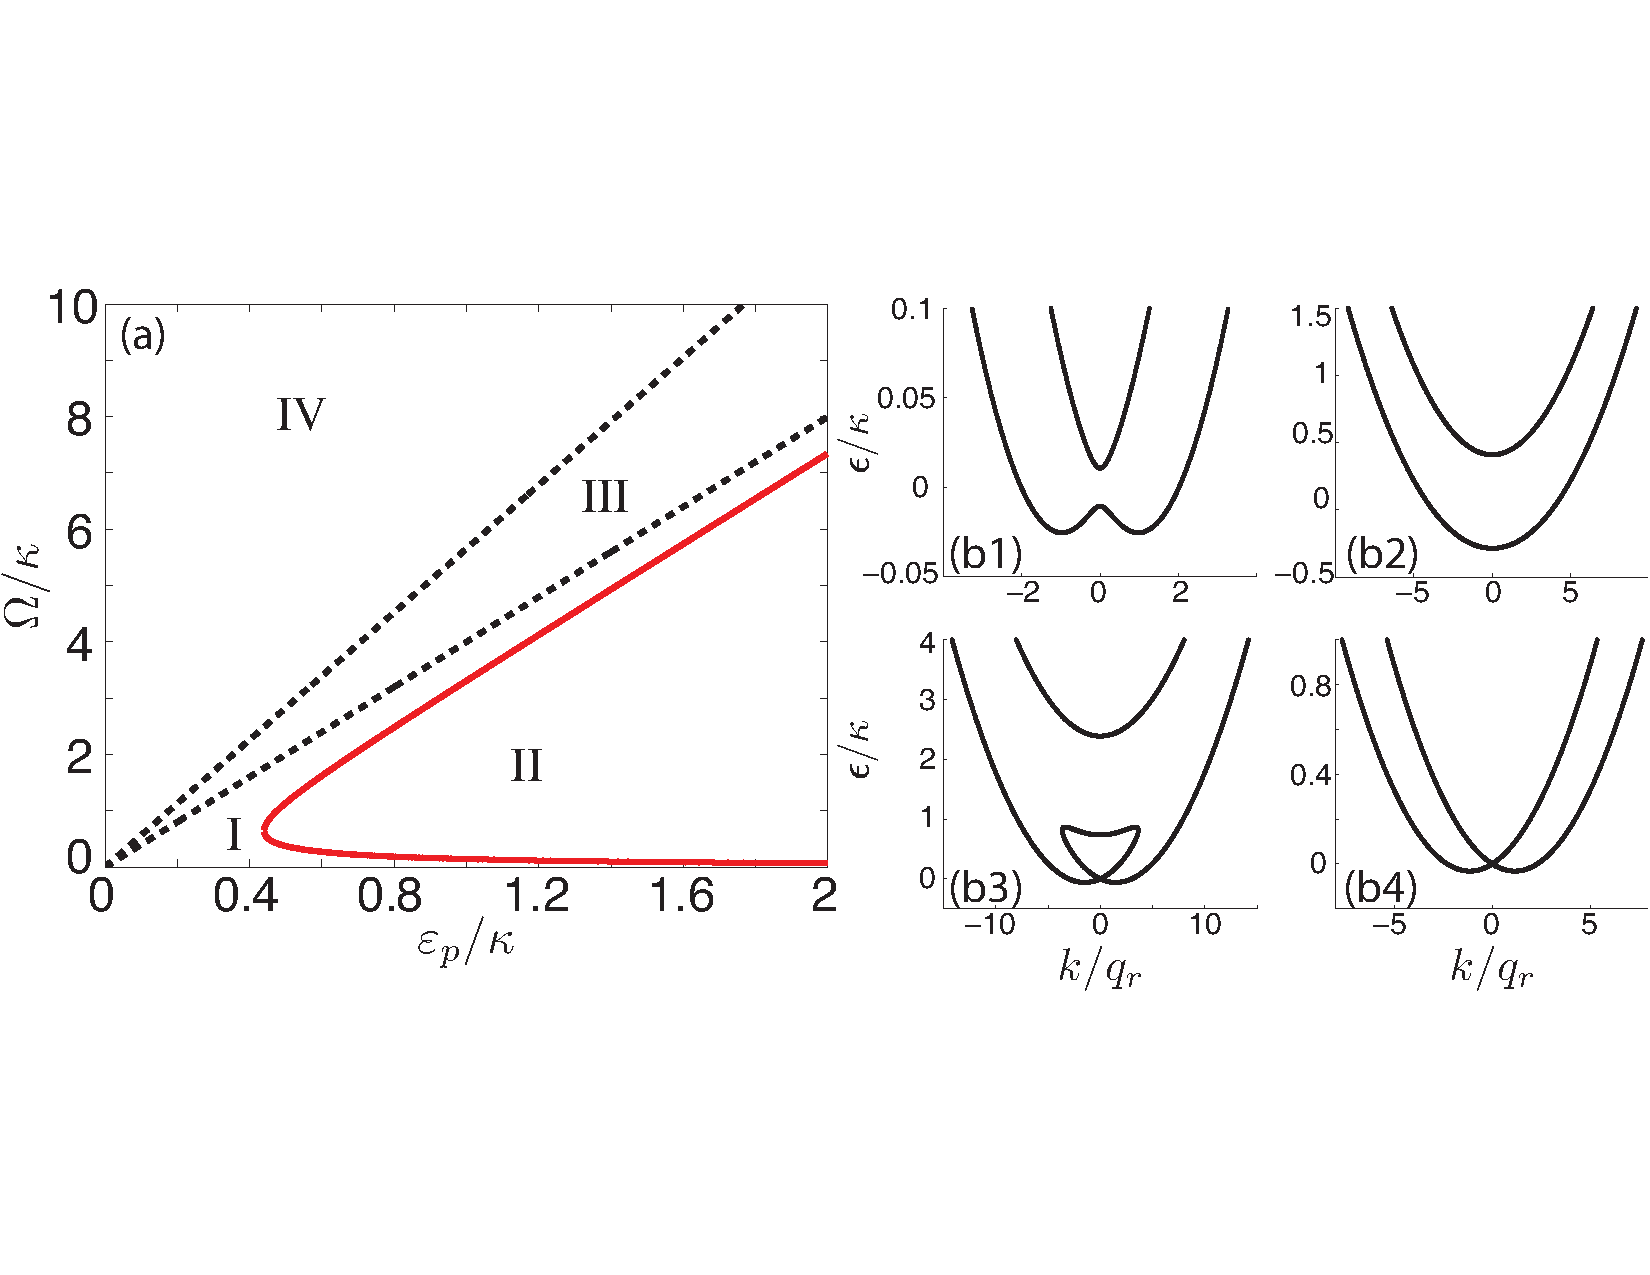
\includegraphics[width=\textwidth]{fig1}\caption{ Single particle eigen-energy spectrum ``phase diagram''. For given paramter $\delta_c=\kappa$ and $\delta=0$, the dispersion behavior is catagorized into four regions, represented from I to IV in (a). From (b1) to (b4), we fix $\varepsilon_p=\kappa$. In region I, the dispersion has double minima as shown in (b1) with $\Omega=0.03\kappa$; region II is enclosed by the red solid curve in (a) and we show the typical point in (b2) ($\Omega=\kappa$) where only single minimum exisits in the lower helicity band; region III is enclosed by the black dashed lines in (a) and it is a region where loop structure emerge, as in (b3) with $\Omega=5\kappa$; finally, in region IV we recover the double minimum dispersion although it's different from region I by closing the gap at $k_z=0$, as in (b4) with $\Omega=8\kappa$.}\label{fig1}
\end{figure}

From the Hamiltonian~(\ref{effH}), one can easily obtain the EOM in Heisenberg picture. To make progress, we adopt the mean-field approximation by replacing the operators by their respective expectation values: $c \rightarrow \langle c \rangle \,, \psi_\sigma ({\bf r}) \rightarrow \langle \psi_\sigma ({\bf r}) \rangle \equiv \varphi_\sigma ({\bf r})$. 
%The mean-field approximation is justified by assuming small quantum fluctuations of both operators $c$ and $\psi_\sigma({\bf r})$. 
Assuming spatial homogeneity, we further take the plane-wave wave-function for the atomic modes $\varphi_\sigma({\bf r})=e^{i{\bf k}\cdot{\bf r}}\varphi_\sigma$ with the normalization condition $|\varphi_\uparrow|^2+|\varphi_\downarrow|^2=\mathcal{N}$. The steady-state solution for the photon field is obtained by taking the time derivative of the photon field to be zero, which is exact by itself without making further approximations. After some algebra, we write the coupled nonlinear time-dependent equations for the two spin components as, 
\ba
i\dot{\varphi}_{\uparrow}&\!\! =\!\! & \left(\frac{{\bf k}^{2}}{2m}+q_{r}k_{z}+\delta\right) \varphi_{\uparrow}+\frac{\Omega}{2}\frac{\varepsilon_{p}-i\frac{\Omega}{2} \mathcal{N}\varphi_\downarrow^\ast\varphi_\uparrow}{\kappa-i\delta_{c}}\varphi_{\downarrow} \,,\label{EOMphi1}\\
i\dot{\varphi}_{\downarrow} & \!\!= \!\!& \left(\frac{{\bf k}^{2}}{2m}-q_{r}k_{z}-\delta\right)\varphi_{\downarrow}+\frac{\Omega}{2}\frac{\varepsilon_{p}+i\frac{\Omega}{2} \mathcal{N}\varphi_\uparrow^\ast\varphi_\downarrow}{\kappa+i\delta_{c}}\varphi_{\uparrow}\,.\label{EOMphi2}
\ea

For a given atomic quasi-momentum ${\bf k}$, we define eigenstate and eigenenergy as the solution of the time-independent version of Eqs.~(\ref{EOMphi1}) and (\ref{EOMphi2}),  by replacing $i(\partial/\partial t)$ with $\epsilon({\bf k})$. We consider $\mathcal{N}=1$ and always take $k_x =k_y=0$ hereafter. After some lengthy nonetheless straightforward algebra, we find that $\epsilon({\bf k})$ obeys a quartic equation
% (we consider $\mathcal{N}=1$ hereafter): 
\begin{equation}
4\epsilon^4+B\epsilon^3+C\epsilon^2+D\epsilon+E=0 \,,
\label{generalquarticEq}
\end{equation}
where detailed derivations are better elaborated in the Supplementary Material of \cite{cavitySOC}. 
%In principle, the quartic equation
%~(\ref{generalquarticEq}) 
%can be solved analytically, but the expressions are too cumbersome to give any physical insights. 
%We plot the typical behavior of the dispersion relation $\epsilon({ k_z})$ vs $k_z$ for $\delta=0$ in Fig.~\ref{atomloops}.
% Note that we always take $k_x =k_y=0$, as the SOC only occurs along the $z$-axis. 
%We found a loop structure develops in the dispersion curve, where a maximum of four real roots are allowed by the quartic equation. 
%Eq.~(\ref{generalquarticEq}). 
%As we will show, in such regimes, a loop structure develops in the dispersion curve.
%As shown in Fig.~\ref{atomloops}, for $\delta_c=0$ (i.e., the pump field is resonant with the cavity), we always have two dispersion branches. The two branches are gapped when the atom-photon coupling strength $\Omega$ is small and touch each other at $k_z=0$ when $\Omega$ exceeds a critical value. For $\delta_c \neq 0$, we again have two gapped branches at small $\Omega$. As $\Omega$ is increased beyond a critical value, a loop appears near $k_z=0$ in either the upper or the lower branch depending on the sign of $\delta_c$. The loop increases in size as $\Omega$ increases and finally touches the other branch and dissolves when $\Omega$ reaches a second critical value. Note that such a dispersion relation is markedly different from that without the cavity, in which case one always obtains two gapped branches. The dispersion curves for finite $\delta$ are qualitatively similar, but in that case the curves are no longer symmetric about $k_z=0$ and the loop emerges  at finite $k_z$. 

We can gain some insights about the general structure of the dispersion relation $\epsilon({\bf k})$, e.g. the degeneracy condition and the appearance and disappearance of the loop. 
%We examine the roots to the quartic equation for $k_z=0$ and $\delta=0$, where it is simplified to a quadratic one  \cite{cavitySOC}. 
%Under these conditions, Eq.~(\ref{generalquarticEq}) is simplified to:
%\begin{equation}
%\epsilon^2(4\epsilon^2-2w\epsilon+|v|^2-4|u|^2)=0\,,
%\label{simplequartic}
%\end{equation}
%with the constraint that the root $\epsilon=0$ is only valid for $\Omega \ge 4\epsilon_p$ (For $\Omega<4\epsilon_p$, the solution $\epsilon=0$ corresponds to trivial state with $\varphi_\uparrow=\varphi_\downarrow=0$.).
%Here the coefficients $w$, $u$ and $v$ are defined in the Supplementary Material of \cite{cavitySOC}. 
Simple analysis shows that there should be a total of four regimes. 
%(i) When $0<\Omega<\Omega_c^{(0)}$, we have two real roots with degenerate lowest eigenenergy at $\pm k_z$ values. In principle, we could examine the change of sign for $d^2\epsilon(k_z)/dk_z^2$ at $k_z=0$ and express $\Omega_c^{(0)}$ as a function of various system parameters analytically. But the expressions are too cumbersome to give any physical insights. Hence, in Fig.~\ref{fig1}, we show ...  
(i) As denoted by region I in Fig.~\ref{fig1}(a) and (b1), we show the dispersion curve exhibits a double minima structure. What is different from the degenercy condition given by the classical laser induced SOC Hamiltonian, is that for arbitrarily small $\Omega$, there {\em always} are double minima in the dispersion. 
%(ii) When $\Omega_c^{(0)} < \Omega <4\varepsilon_p\equiv\Omega_c^{(1)}$, we have a non-degenerate single minimum solution and the quartic equation gives two real roots, one positive and one negative. 
%This corresponds to the two gapped branches for small $\Omega$. 
(ii) In region II of Fig.~\ref{fig1}(a) and (b2), the dispersion curve has only single minimum. 
(iii) Region III corresponds to the region with loop structure and in Fig.~\ref{fig1}(a) the two dashed black line are numerically obtained by examining the sign of second order derivative of the root with respect to $k_z$. When $\Omega_c^{(1)}\equiv4\varepsilon_p\leq \Omega \leq  4\varepsilon_p \sqrt{1+(\delta_c/\kappa)^2}\equiv\Omega_c^{(2)}$, at $k_z=0$ there are total of four real roots allowed by the quartic equation --- two degenerate roots at $\epsilon=0$ and two additional roots with the same sign, see for instance Fig.~\ref{fig1}(b3). 
%It also agrees with the analytic expression for $\Omega_c^{(1)}$ and $\Omega_c^{(2)}$ as a function of $\varepsilon_p$. 
%This corresponds to the looped regime in the middle row of Fig.~\ref{atomloops}. 
(iv) Finally, when $\Omega > \Omega_c^{(2)}$ in region IV, only the two degenerate roots at $\epsilon(k_z=0)=0$ exist and we show the double minimum dispersion curve and gapless point at $k_z=0$, see (b4) for instance.  
%, which correspond to the gapless regime represented by the bottom row in Fig.~\ref{atomloops}. 
% Note that for $\delta_c=0$, we have $\Omega_c^{(1)}=\Omega_c^{(2)}=4\epsilon_p$, and the loop never develops, nonetheless degeneracy condition still holds as {\color{red} bla bla bla and bla}. 

The re-entrant behavior of the dispersion degeneracy can be understood by considering the effective Raman coupling strength $|\Omega_\text{eff}|\equiv\frac{\Omega}{2}\left|\frac{\varepsilon_{p}-i\frac{\Omega}{2}\varphi_\downarrow^\ast\varphi_\uparrow}{\kappa-i\delta_{c}}\right|$. To this end, in Fig.~\ref{fig2}(a) we plot $|\Omega_\text{eff}|$ as a function of $\Omega$ for different $k_z$ values (for illustration purposes we have chosen the lowest eigen-energy branch to compute the wave-functions $\varphi_\uparrow$ and $\varphi_\downarrow$). We note that $|\Omega_\text{eff}|$ does not monotonically increase with $\Omega$, but rather to increase to a maximum and decrease back to zero at large $\Omega$ limit. This is once again due to the dynamic feedback of photon field onto atom center degrees of freedom. At small limit of $\Omega$, atom-photon coupling is weak and atomic states with different $k_z$ behave universally the same so that the atom photon field is effectively decoupled, which can be evidenced from the same linear slope $d|\Omega_\text{eff}|/d\Omega$ in the small $\Omega$ limit. On the other hand, when $\Omega$ becomes exceedingly large, such that photon is blocked away from entering the cavity (known as photon blockade), effective coupling between atom and photon is rather small and atomic bare spin state dominates over dressed state basis. In between these two limits, the re-entrant behavior of degenerate and non-degenerate dispersion is manifested in terms of $|\Omega_\text{eff}|$'s non-monotonousness as a function of $\Omega$.

%The emergence of the loop structure is a distinctive nonlinear feature of the system. We remark that similar loop structures or the associated hysteretic phenomena have been found in other nonlinear systems \cite{sup}. The nonlinearity may originate from the mean-field density-density interaction \cite{loopPapers} or from the cavity-induced feedback between atoms and photons \cite{loop1}. The case studied here corresponds to the latter situation. However, in previous studies of ``ultracold atom + cavity" systems \cite{loop1}, the interaction between the cavity photons and atoms is dispersive, and so it does not induce SOC directly. As we will show below, the system studied here possesses very different dynamical and stability properties.   

We remark that the introduction of cavity photon feedback dramatically alters the dispersion relation, where one we could obtain from current proposals concerning classical laser induced SOC setups. As a matter of fact, due to cavity mediation, the emergent loop structure is a distinctive nonlinear feature of the system. Furthermore, upon studying the linearized perturbative expansion on top of fixed point solution to Eq.~\ref{EOMphi1} and Eq.~\ref{EOMphi2}, we have found intriguing dynamical stability properties, where there {\em always} exist both dynamically stable and unstable branches regardless whether there is loop or not \cite{cavitySOC}. Nonetheless, if we consider the large limit of pumping rate $\varepsilon_p$, we will again be able to recover classical laser induced SOC limit. In this scenario, cavity photon field becomes the coherent state and atomic dressed state appears as bare spin state such that $|\Omega_\text{eff}|\rightarrow\frac{\Omega}{2}\frac{\varepsilon_p}{\sqrt{\kappa^2+\delta_c^2}}$ in this limit. Then one can recover the degeneracy condition for classical laser induced SOC Hamiltonian. When $\Omega<4E_r\frac{\sqrt{\kappa^2+\delta_c^2}}{\varepsilon_p}$ dispersion curve has degenerate double minimum; When $\Omega>4E_r\frac{\sqrt{\kappa^2+\delta_c^2}}{\varepsilon_p}$ we only have a single minimum in the dispersion curve. As we show in Fig.~\ref{fig2}(b), the cavity-assisted SOC determined boundary curve asymptotically approaches the blue dashed line which is given by the classical correspondence of large pumping rate limit of  $4E_r\frac{\sqrt{\kappa^2+\delta_c^2}}{\varepsilon_p}$. Note, in large $\varepsilon_p$ limit, dynamical instability decay rate $\gamma$ is also strongly suppressed to a small value, such that the system fully recovers the classical laser induced SOC Hamiltonian. 

\begin{figure}[htp]
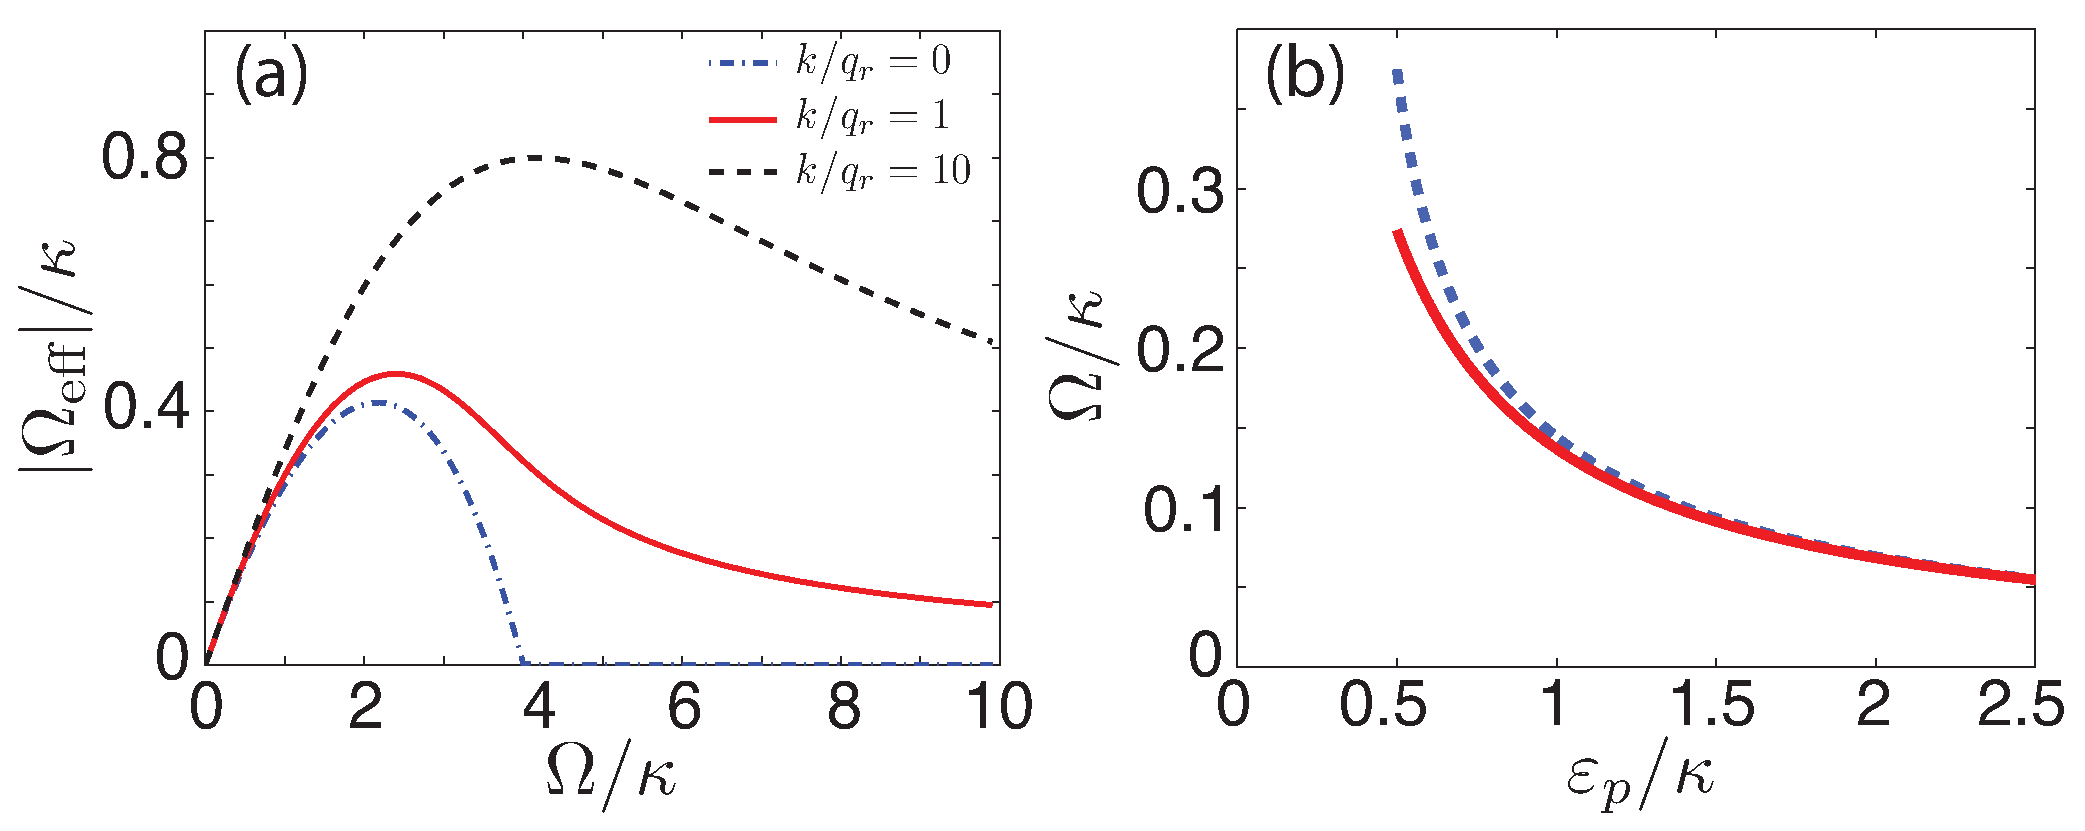
\includegraphics[width=0.95\textwidth]{fig2}\caption{(a) Effective Raman coupling $|\Omega_\text{eff}|$ is plotted as a function of atom-photon coupling strength $\Omega$ for different $k_z$ values, $0$,\,$q_r$,\,$10q_r$ for blue dash-dot, red solid and black dashed  lines. We observe that $|\Omega_\text{eff}|$ does not monotonically  increases with $\Omega$ but rather peaks at an intermediate value, then approaches zero in the large $\Omega$ limit. Figure (b) shows a comparison between critical boundary of region I and II (red curve) and large pumping rate limit of $|\Omega_\text{eff}|$ (blue dashed line). At large $\varepsilon_p$ limit, the two results match asymptotically well.  }\label{fig2}
\end{figure}

As we will also emphasize in Sec.~\ref{relation}, the synthesis of cavity confinement and Raman coupling is not a trivial combination, but rather gives rise tonontrivial physics that deserves more scrutiny. In order to better address the intricate coupling between atom and photon, we dedicate the Sec.~\ref{master} and Sec.~\ref{relation} to explore more on the quantum nature of this system. 

\section{Master Equation Approach: Full Quantum Mechanical Treatment } \label{master}

Semi-classical mean field approach gives an intuitive picture of understanding the atom-light interaction, as we have shown above. However, it ignores quantum fluctuations of both operators $c$ and $\psi_\sigma({\bf r})$. A more stringent approach is given by solving quantum master equation.
%, which is especially useful to study few cavity photon scenario. 
The quantum master equations, in a nutshell, are differential equations for the density operators, including contributions from off-diagonal elements which represents quantum coherence characteristically.
%as a characteristic quantum mechanical signature. 
Master equation is generally considered to be more general than the Schr\"{o}dinger equation, since it uses the density operator instead of a specific state vector and can therefore give statistical as well as quantum mechanical information. 

Instead of treating the leakage of cavity photon phenomenologically in Eq.~(\ref{effH}), we model the dissipation process by Liouvillean terms $\mathcal{L}$ appearing in the Lindblad master equation for the atom-field density operator, i.e., 
\be 
\dot{\rho} = \frac{1}{i\hbar}[H_{\text{eff}},\rho]+\mathcal{L}\rho \,. \label{masterEq}
\ee
where $H_{\text{eff}}$ is the same as $\mathcal{H}_{\text{eff}}$ in Eq.~(\ref{effH}) by dropping the last term, i.e. $-i\kappa c^{\dagger}c$. Cavity loss is accommodated by the standard form of Lindblad superoperator \cite{L1, L2},
\be 
\mathcal{L}\rho = \kappa (2c\rho c^\dagger-c^\dagger c\rho-\rho c^\dagger c)\,.\label{Lindblad}
\ee
Again, due to spatial homogeneity, we decouple momentum eigenstates by taking the plane-wave ansatz for the atomic modes as $\varphi_\sigma({\bf r})=e^{i{\bf k}\cdot{\bf r}}\varphi_\sigma$. Thereon, we are granted to work under the Hilbert subspace of a given momentum value ${\bf k}$. Here we explicitly write the commutator as,
\ba
[H_{\text{eff}}({\bf k}),\rho] & = & \left(\frac{{\bf k}^{2}}{2m}+\frac{q_{r}k_{z}}{m}+\delta\right)\left(\varphi_{\uparrow}^{\dagger}\psi_{\uparrow}\rho-\rho\varphi_{\uparrow}^{\dagger}\psi_{\uparrow}\right)+\left(\frac{{\bf k}^{2}}{2m}-\frac{q_{r}k_{z}}{m}-\delta\right)\left(\psi_{\downarrow}^{\dagger}\varphi_{\downarrow}\rho-\rho\varphi_{\downarrow}^{\dagger}\varphi_{\downarrow}\right)\nonumber\\
 & + & \mathcal{N}\frac{\Omega}{2}\left(\varphi_{\uparrow}^{\dagger}\varphi_{\downarrow}c\rho+c^{\dagger}\varphi_{\downarrow}^{\dagger}\varphi_{\uparrow}\rho-\rho\varphi_{\uparrow}^{\dagger}\varphi_{\downarrow}c-\rho c^{\dagger}\varphi_{\downarrow}^{\dagger}\varphi_{\uparrow}\right)\nonumber\\
&+&i\varepsilon_{p}\left(c^{\dagger}\rho-c\rho-\rho c^{\dagger}+\rho c\right)-\delta_{c}\left(c^{\dagger}c\rho-\rho c^{\dagger}c\right)\,.
\ea
To solve the operator equation, Eq.~\ref{masterEq}, we choose our basis state as direct product state $|n;\sigma\rangle$, %$n=0,1,2,...,\infty$ 
where non-negative integer $n$ denotes photon number 
%and $N$ is the truncation number of photon inside the cavity 
and atomic pseudo-spin state is represented by $\sigma=\uparrow,\downarrow$. Our goal is to calculate the entire matrix elements of density operator under this set of basis states, denoted by $\langle m;\sigma|\rho|n;\sigma'\rangle\equiv\rho_{mn}^{\sigma\sigma'}$. Without loss of generality, we have taken atom number $\mathcal{N}=1$ to simplify discussions. We found the governing EOM can be written as,
\ba 
\frac{d}{dt}\rho_{mn}^{\sigma\sigma'} 
& = & -i\left(\frac{{\bf k}^{2}}{2m}+\frac{q_{r}k_{z}}{m}+\delta\right)\left(\delta_{\sigma\uparrow}-\delta_{\sigma'\uparrow}\right)\rho_{mn}^{\sigma\sigma'}
-  i\left(\frac{{\bf k}^{2}}{2m}-\frac{q_{r}k_{z}}{m}-\delta\right)\left(\delta_{\sigma\downarrow}-\delta_{\sigma'\downarrow}\right)\rho_{mn}^{\sigma\sigma'}\nonumber\\
& + & \frac{\Omega}{2i}(\delta_{\sigma\uparrow}\sqrt{m+1}\rho_{m+1n}^{\bar{\sigma}\sigma'}
+\delta_{\sigma\downarrow}\sqrt{m}\rho_{m-1n}^{\bar{\sigma}\sigma'}
-\delta_{\sigma'\uparrow}\sqrt{n+1}\rho_{mn+1}^{\sigma\bar{\sigma'}}
-\delta_{\sigma'\downarrow}\sqrt{n}\rho_{mn-1}^{\sigma\bar{\sigma'}})\nonumber\\
& + & \varepsilon_{p}\left(\sqrt{m}\rho_{m-1n}^{\sigma\sigma'}-\sqrt{m+1}\rho_{m+1n}^{\sigma\sigma'}+\sqrt{n}\rho_{mn-1}^{\sigma\sigma'}-\sqrt{n+1}\rho_{mn+1}^{\sigma\sigma'}\right)\nonumber\\
& + & i\delta_{c}\left(m-n\right)\rho_{mn}^{\sigma\sigma'}
+ \kappa\left(2\sqrt{m+1}\sqrt{n+1}\rho_{m+1n+1}^{\sigma\sigma'}-(m+n)\rho_{mn}^{\sigma\sigma'}\right),\label{EOMrho}
\ea
where $\bar{\sigma}$ represents the flip-spin value, i.e. $\bar{\uparrow}=\downarrow$ and $\bar{\downarrow}=\uparrow$. 

With Eq.~\ref{EOMrho}, we can study dynamical evolution of density operator $\rho$ for a given initial state. For instance, we can initiate the system with a pure state $|0;\uparrow\rangle$, construct density operator $\rho=|0;\uparrow\rangle\langle0;\uparrow|$, and let it evolve according to Eq.~\ref{EOMrho} until all components reach their respective steady state. Although at $t=0$ we have $\text{Tr}[\rho^2]=1$, at later times, we will always have $\text{Tr}[\rho^2]<1$ for nonzero $\kappa$, because cavity decay term renders the system into mixed states. 

Assuming the fate of time evolution gives the steady state solution, we can also solve the set of equations after equating the RHS of Eq.~\ref{EOMrho} to zero. Numerically, this is achieved by introducing a large truncation value $N$ for maximum number of cavity photon under consideration, such that the problem reduces to simple linear algebra manipulations. In the following, we mainly focus on the steady-state solution of density operator and ignore the transient dynamics.

In order to further quantitatively characterize atom-photon interaction in this open system, we invoke the entanglement measure for mixed-state, the so-called negativity \cite{negativity}, defined as $\mathcal{N}(\rho)=\frac{||\rho^{T_A}||_1-1}{2}$, where $||\rho^{T_A}||_1$ denotes the trace norm of partial transpose of density operator with respect to atom party (the same is true for photon party). Density matrix $\rho$ itself gives all positive definite eigenvalues and thus the trace norm $||\rho||_1=\text{Tr}[\sqrt{\rho^\dagger\rho}]=\text{Tr}[\rho]=1$. Although the partial transpose $\rho^{T_A}$ still satisfies $\text{Tr}[\rho^{T_A}]=1$, it does not necessarily guarantee positive definiteness in eigenvalues. The trace norm is written generally as $||\rho^{T_A}||_1=1+2\sum_i|\mu_i|$ where we have denoted negative eigenvalues as $\mu_i<0$. Thus, by definition, the negativity $\mathcal{N}(\rho)$ is equal to $\sum_i|\mu_i|$ 
%-- the absolute sum of negative eigenvalues $\mu_i$ of $\rho^{T_A}$
, which measures by how much $\rho^{T_A}$ fails to be positive definite. An immediate consequence for any separable (unentangled) state $\rho_s$ is that $\mathcal{N}(\rho_s)=0$, while for unseparable mixed state, $\mathcal{N}(\rho)$ is believed to be a good entanglement measure. 

\section{Results and Discussions} \label{relation}

With above preparations, we are now in a position to discuss about the results given by the two approaches, and address their relationship. As we have shown above and also in previous work \cite{cavitySOC}, the cavity feedback dramatically modifies single particle dispersion relation. For instance, in intermediate region of atom-photon coupling strength of $\Omega$, a loop structure emerge from the center tip of the eigenenergy spectrum. Additionally, in this effective nonlinear system, although atom-photon coupling is linear, dispersion spectrum possesses intriguing stability/instability properties. What we have shown in \cite{cavitySOC} also indicates that only part of the dispersion is stable for a given quasi-momentum state ${\bf k}$. The instability analysis prescribes a recipe to map out regions whether fluctuations around fixed point solution would grow exponentially or not. Tout de suite, we apply the formalism developed in Sec.~\ref{meanfield} and Sec.~\ref{master} to calculate photon number expectation value inside the cavity.

\begin{figure}[htp]
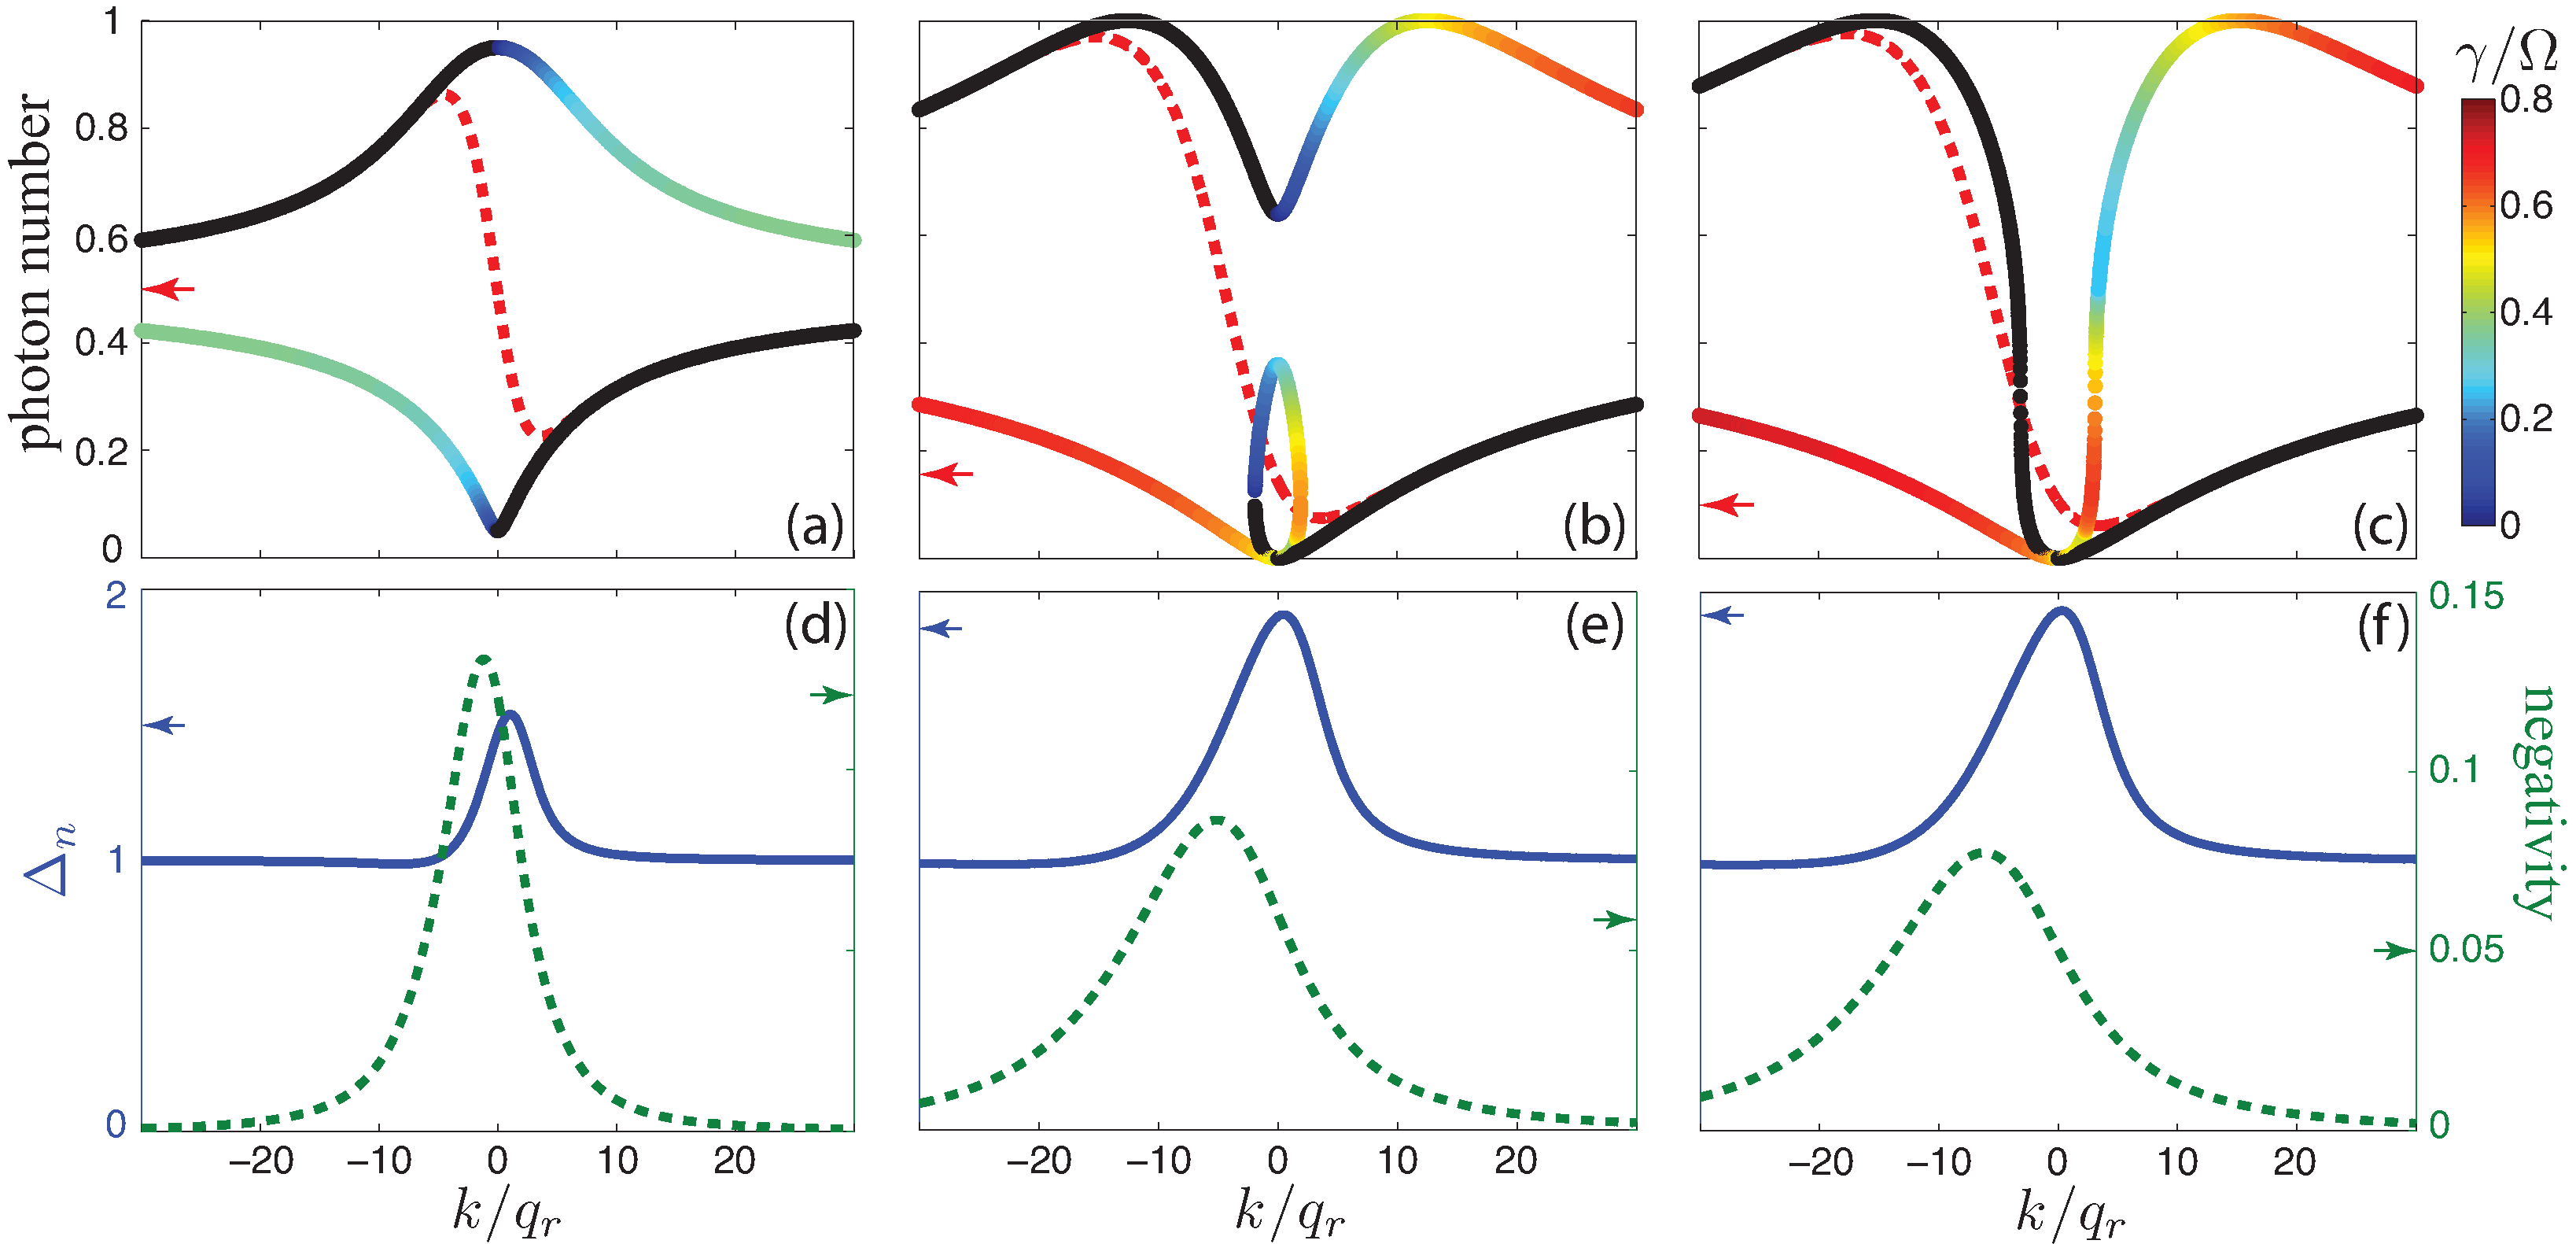
\includegraphics[width=0.95\textwidth]{photon}
\caption{ Photon number comparison between semi-classical mean field result and full quantum mechanical master equation solution. From (a) to (c), $\Omega = 3\kappa,\ 5.6\kappa,\ 6\kappa$ and colorbar represents the renormalized decay rate $\gamma/\Omega$ of unstable states and red dashed lines are master equation solutions. Figures from (d) to (f) show the corresponding photon number fluctuation (blue solid curve) and negativity (green dashed line). Other parameters are $\varepsilon_p=\kappa$, $\delta_c=\kappa$, $\delta=0$ and $\kappa=1$ in the dimensionless unit. Although we have chosen $q_r=0.22$ in our units (based on a realistic experimental parameter estimate) throughout all figures, we use arrows on vertical axis to denote results concerning $q_r=0$ limit. 
%At the large $k_z$ limit, we found $\text{Tr}[\rho_\text{photon}n]$ asymtotes to semi-classical mean field result $|\langle c\rangle|^2$, which further matches stable branches according to mean field stability analysis.
}
\label{photon}
\end{figure}

As we show in Fig.~\ref{photon}(a)-(c), we plot semi-classical mean field  photon number $|\langle c\rangle|^2$ and quantum mechanical master equation result $\text{Tr}[\rho n]$, against atom's dimensionless quasi-momentum $k_z/q_r$. From semi-classical mean field result, with increasing magnitude of $\Omega$, we sweep over regions with only two real roots, four real roots and only one double root (at $\epsilon=0$) to the mean field solution of the quartic equation. We can further perform dynamical analysis \cite{cavitySOC} to pinpoint stable (black dots) and unstable branches of the semi-classical solution. For unstable states, we use colorbar to denote the renormalized decay rate $\gamma/\Omega$ where $\gamma$ refers to the largest real eigenvalue of perturbed dynamical equation \cite{cavitySOC}. 
%We found for any set of parameters and given $k_z$ value, we always have dynamically stable and unstable branches, regardless whether there is loop or not. This is rather surprising since it shows that the cavity back-action completely modifies the system's stability properties.
For comparison, with the same parameter set, we start from quantum master equation Eq.~\ref{EOMrho}, and obtain steady state solution of density operator, and trace over the product of density operator and photon number, i.e. $\langle n\rangle=\text{Tr}[\rho n]$. Unlike semi-classical mean field theory, we can only have one unique solution of steady state density operator, thus only one branch of average photon number is found as a function of $k_z$, as represented by the red dashed line in  Fig.~\ref{photon}(a)-(c).

We found, remarkably, that $\text{Tr}[\rho n]$ asymptotically approaches $|\langle c\rangle|^2$ value in dynamically stable branches at large $|k_z|$ limit. 
%Several observations are in order. 
This agreement, first of all, further validates our previous dynamical stability analysis of semi-classical mean field result \cite{cavitySOC}. Due to momentum exchange of $\pm2\hbar q_r\hat{z}$ in the Raman process, atomic states with small quasi-momentum $|k_z|$ are more coupled with photon field, in comparison to the states with large  $|k_z|$. One would have naively thought cavity-assisted SOC should naturally provide more coupling between atom and photon field than the system with synthetic SOC, because atomic pseudo-spin state and COM are both coupled to cavity photon here. However, it is the SOC that renders this coupling {\em depends} on atomic quasi-momentum: (i) Momentum exchange plays a major role at small $k_z$ where two SOC bands are avoided-crossing, and eigenstate is a strong hybridization between bare atomic pseudo-spin states. Thus atom and photon is strongly coupled in this region. (ii) While at large $k_z$ limit, energy separation becomes so large that the two dressed states are more like two independent bare atomic pseudo-spin states $|\uparrow\rangle$ and $|\downarrow\rangle$. Atomic spin state, COM and photon field are all decoupled in this limit. 
 
Second, 
% at large $|k_z|$ value, master equation solution asymptotically collapes onto mean field solution, which 
the relationship between semi-classical mean field result and quantum master equation result can be understood from photon number fluctuation, which by definition is given by $\frac{\langle(\Delta n)^{2}\rangle}{\langle n\rangle}=\frac{\langle n^{2}\rangle-\langle n\rangle^{2}}{\langle n\rangle}$. In Fig.~\ref{photon}(d)-(f), on the left $y$-axis, we plot the renormalized fluctuation magnitude as a function of $k_z$, shown as blue solid curve. We found it degrades to one in large $|k_z|$ limit, and this is the limit where photon state is best modeled by the coherent state (Poissonian statistics) and atom's back-action {\em onto} photon becomes negligibly small. 
For small $|k_z|$ values, the majority part of fluctuation is larger than one, which implies a super-Poissonian photon number distribution, where cavity photon behaves more thermal like, which is far away from coherent state. If we have a  positive definite probability distribution for photon number, by the application of Cauchy-Schwarz inequality, the fluctuation value would always have to be greater or equal to one. However, there are regions where renormalized fluctuation is smaller than one, e.g. in Fig.~\ref{photon}(d) at small negative $k_z$ value,  $\frac{\langle(\Delta n)^{2}\rangle}{\langle n\rangle} \sim 0.95$, which implies sub-Poissonian photon number distribution as a signature of system being genuinely non-classical. 

Third, the degree of entanglement for a mixed-state can be quantitatively characterized by the negativity $\mathcal{N}(\rho)$ \cite{negativity}, which we briefly mentioned in Sec.~\ref{master}. In Fig.~\ref{photon}(d)-(f), on the right $y$-axis, we plot the negativity against $k_z/q_r$ for different $\Omega$ values using green dashed lines. We can see that when photon field approaches its coherent state at large $|k_z|$, negativity becomes very close to zero which means the ``atom + photon'' system becomes separable. When photon fluctuation deviates from one, negativity shows up a pronounced peak in a qualitatively similar manner. 
%Despite the fact the two curves' peak centers at different $k_z$ value, one could still conclude that when atom and photon field is more entangled, photon number distribution deviates further away from Poissonian distribution. 

%Third, there are regions where renormalized fluctuation is smaller than one, e.g. in Fig.~\ref{photon}(d) at small negative $k_z$ value,  $\frac{\langle(\Delta n)^{2}\rangle}{\langle n\rangle} \sim 0.95$, which implies sub-Poissonian photon number distribution as a signature of system being genuinely non-classical. For the majority part, we have $\frac{\langle(\Delta n)^{2}\rangle}{\langle n\rangle}>1$ (super-Poissonian distribution), which leads to bunched spacing according to the statistics, i.e. more thermal like. In other words, ``slow'' atomic states have larger probabilities of back scattering cavity photon and photon field thus becomes more entangled and behaves like a source of chaotic light. It can be shown by the application of Cauchy-Schwarz inequality, the fluctuation term would have to be greater or equal to one, if we have a positive definite probability distribution for photon number. But it seems in our system, the photon number probability does not necessarily has to be greater than zero. ({\color{red} we can perhaps straightforwardly demonstrate this by plotting $p(n)=\langle n|\hat{\rho}_{\text{photon}}|n\rangle$ where $\hat{\rho}_{\text{photon}}$ is the reduced density matrix for photon by tracing over atomic degrees of freedom in total density opeartor, i.e. $\rho_{\text{photon}}=\text{Tr}_{\text{atom}}[\rho]$. For coherent light, $p_{\text{coh}}(n)=\frac{\langle n\rangle^{n}}{n!}e^{-\langle n\rangle}$; and for thermal light, $p_{\text{th}}(n)=\frac{1}{1+\langle n\rangle}(\frac{\langle n\rangle}{1+\langle n\rangle})^{n}$. I have tested small pumping rate $\varepsilon_p$ gives better fit of $p(n)$ to  $p_{\text{th}}(n)$ and for large value of $\varepsilon_p$, $p(n)$ is closer to $p_{\text{coh}}(n)$.})

%After we have the steady state solution of total system's density operator, we can compute expectation value of photon number operator by tracing over the product, i.e. $\langle n\rangle=\text{Tr}[\rho n]=\rho_{nn}^{\uparrow\uparrow}+\rho_{nn}^{\downarrow\downarrow}$ and  photon number fluctuation $\frac{\langle(\Delta n)^{2}\rangle}{\langle n\rangle}=\frac{\langle n^{2}\rangle-\langle n\rangle^{2}}{\langle n\rangle}$. 
%As we show in Fig.~\ref{photon}, $\text{Tr}[\rho n]$ deviates from $|\langle c\rangle|^2$ at small $|k_z|$ value, where normalized fluctuation term is larger than one (super-Poissonian distribution). This mean cavity photon prefers to have bunched spacing according to the statistics, i.e. more thermal like. In other words, ``slow'' atomic states have larger probabilities of back scattering cavity photon and photon field thus becomes more entangled and behaves like a source of chaotic light.
% {\color{red} better interpretation?} 
%However, when we are in the large limit of  $|k_z|$, quantum results asymtopically approaches semi-classical mean field solution, while fluctuation magnitude uniformly degrades to unit one. This is the limiting case where photon statistics is best modeled by the coherent state (Poissonian statistics), where atom's back-action {\em onto} photon becomes negligibly small. And, semi-classical mean field theory agrees with quantum master solution in this limit. 
% {\color{red} better interpretation?}

%We can also consider the probability of finding $n$ photon, defined as $p(n)=\langle n|\hat{\rho}_{\text{photon}}|n\rangle$ where $\hat{\rho}_{\text{photon}}$ is the reduced density matrix for photon by tracing over atomic degrees of freedom in total density opeartor, i.e. $\rho_{\text{photon}}=\text{Tr}_{\text{atom}}[\rho]$. For coherent light, $p_{\text{coh}}(n)=\frac{\langle n\rangle^{n}}{n!}e^{-\langle n\rangle}$; and for thermal light, $p_{\text{th}}(n)=\frac{1}{1+\langle n\rangle}(\frac{\langle n\rangle}{1+\langle n\rangle})^{n}$. We have found small pumping rate $\varepsilon_p$ gives better fit of $p(n)$ to  $p_{\text{th}}(n)$ and for large value of $\varepsilon_p$, $p(n)$ is closer to $p_{\text{coh}}(n)$. Since we always have a positive definite probability distribution for photon number, the fluctuation term would have to be greater or equal to one, which can be shown by an application of the Cauchy-Schwarz inequality.
 %{\color{red} would there be any region of parameter that gives sub-Possonian field, that are genuinely non-classical feature of quantum optics? Negative Mandel Q parameter, second order intensity correlation function etc.}


%[{\color{red} Rewrite it, simplify it and highlight it.}] Negativity for mixed state is defined as $\mathcal{N}(\rho)=\frac{||\rho^{T_{atom}}||_{1}-1}{2}=\frac{\left(\sum\text{eig}[\rho^{T_{\text{atom}}}]\right)-1}{2}=\sum_{i}\frac{|\lambda_{i}|-\lambda_{i}}{2}$ where $\lambda_{i}$ are all the eigenvalues of $\rho^{T_{atom}}$. Namely, nagativity is the absolute sum of negative eigenvalues of $\rho^{T_{atom}}$, which vanishes for unentangled states. Also, $\rho^{T_{atom}}$ stands for partial transpose of density matrix with respect to atom party, $\rho^{T_{atom}}=\left(\begin{array}{cc} [\rho_{mn}^{\uparrow\uparrow}]^{T} & [\rho_{mn}^{\uparrow\downarrow}]^{T}\\ {}[\rho_{mn}^{\downarrow\uparrow}]^{T} & [\rho_{mn}^{\downarrow\downarrow}]^{T}\end{array}\right)$.

Above observations conclude our discussion on the relationship between semi-classical theory and quantum mechanical master equation approach in the proposed cavity-assisted SOC system. Alternatively, we can also comment on the relationship between cold atom cavity QED physics and the current work. Conventionally, J-C Model is used to describe interaction between a two level atomic state and photon field by ignoring the rest degrees of freedom. In lieu of mimicking J-C Model, we set $q_r$ to zero in the Hamiltonian and repeat the steady state solution to Eq.~\ref{masterEq}. Under this setting, atom's kinetic energy only contribute to a dynamical phase that does not affect expectation value of observable, e.g. photon number, fluctuation, etc. Then we choose an arbitrary value of $k_z$ or ignore $k_z^2/2m$ term altogether, and compute $\text{Tr}[\rho n]$, $\frac{\langle(\Delta n)^{2}\rangle}{\langle n\rangle}$ and $\mathcal{N}(\rho)$ where we use arrows on the $y$-axis to denote their values in Fig.~\ref{photon}. As we can observe in Fig.~\ref{photon} from (a) to (c), photon number in J-C Model limit is very different from the one by considering cavity-assisted SOC, {\em even} in large $k_z$ asymptotic limit. We have $\text{Tr}[\rho n] \approx 0.49,\ 0.14,\ 0.11$ from (a) to (c), while we always have asymptotic value of $\frac{\varepsilon_p^2}{\kappa^2+\delta_c^2}$ {\em independent} of $\Omega$ value in our system, which is $0.5$ in Fig.~\ref{photon}. However, we are able to recover J-C model by simultaneously setting both $q_r$ and $\Omega$ to zero, where there is only generic atomic spin and photon coupling present. In Fig.~\ref{photon} from (d) to (f), we have $\frac{\langle(\Delta n)^{2}\rangle}{\langle n\rangle}\approx1.47,\ 1.91,\ 1.93$ and $\mathcal{N}(\rho)\approx 0.12,\ 0.06,\ 0.05$, respectively.    


\section{Conclusion and Outlook} \label{conclusion}

In this work, we have studied spin-orbit coupled cold atoms inside a ring cavity system, employing both semi-classical mean field theory and full quantum mechanical master equation approach. By treating both light and atom on equal footing and seeking the self-consistent solution in both approaches, we have found cavity-assisted SOC dramatically modified atomic dispersion relation, intriguing dynamical instabilities, and atom's back-action onto light field also leads to non-trivial atom-photon coupling that are fundamentally different to the system with either synthetic SOC or J-C model type of interaction. We have also explored correspondence and discussed the relationship between the two approaches. We conclude that the synthesis of cavity QED and SOC is not a trivial combination and interesting new physics are emergent in this setting. The two distinctively different approaches give us an unified understanding of the atom-light effective non-linearity and induced dynamical instability in this system. 

Although for simplicity reasons we have only considered one atom inside the cavity, the current mean field formalism and results can be easily generalized to $\mathcal{N}$ identical non-interacting bosons, where we would expect similar physics involving atom and light couplings. However, due to anti-symmetrization constraint, for $\mathcal{N}$ non-interacting fermions, it is less straightforward to bridge a connection. Furthermore, it would be interesting to consider atom-atom interactions for the many body case {\color{red} cite Feder's paper here?} and study super-radiant Dicke phase transition {\color{red} cite Hui Zhai's paper and Xiong-Jun Liu's super-radiant paper here?}, using the master equation approach. 

\acknowledgments{Acknowledgments}
We acknowledge discussions with Zhengwei Zhou and XXX. H.P. is supported by the NSF and Welch Foundation (Grant No. C-1669 XXX);
\authorcontributions{Author Contributions}
H.P. conceived the idea of the project, L.D. and C. Z. explored the theoretical and numerical aspects of the physics. All authors contributed to writing and revising the manuscript and participated in the discussions about this work.
\conflictofinterests{Conflicts of Interest}
The authors declare no conflict of interest. 

%=================================================================
% References: Variant A
%=================================================================
% Back Matter (References and Notes)
%----------------------------------------------------------
% Style and layout of the references
% Reference 1
% \bibitem{ref-journal}
% Lastname, F.; Author, T. The title of the cited article. {\em Journal Abbreviation} {\bf 2008}, {\em 10}, 142-149
\bibliographystyle{mdpi}
\makeatletter
\renewcommand\@biblabel[1]{#1. }
\makeatother
\begin{thebibliography}{999} % if there are less than 10 entries, enter a one digit number
\bibitem{JCM}
E.T. Jaynes, F.W. Cummings (1963). Proc. IEEE 51 (1): 89–109. 
\bibitem{exp1987}
G. Rempe, H. Walther, and N. Klein (1987). Phys. Rev. Lett. 58 (4): 353–356.
\begin{comment}
\bibitem{BEC1}
Anderson, M. H., J. R. Ensher, M. R. Matthews, C. E. Wieman, and E. A. Cornell, {\em Science} {\bf 1995}, {\em 269}, 198.
\bibitem{BEC2}
Bradley, C. C., C. A. Sackett, J. J. Tollett, and R. G. Hulet, {\em Phys. Rev. Lett.} {\bf 1995}, {\em 75}, 1687.
\bibitem{BEC3}
Davis, K. B., M.-O. Mewes, M. R. Andrews, N. J. van Druten, D. S. Durfee, D. M. Kurn, and W. Ketterle, {\em Phys. Rev. Lett.} {\bf 1995}, {\em 75}, 3969.
\bibitem{Fermi1}
DeMarco, B., and D. D. Jin, {\em Science} {\bf 1999}, {\em 285}, 1703.
\bibitem{Fermi2}
Truscott, A., K. Strecker, W. McAlexander, G. Partridge, and R. G. Hulet, {\em Science} {\bf 2001}, {\em 291}, 2570.
\bibitem{Fermi3}
Schreck, F., L. Khaykovich, K. L. Corwin, G. Ferrari, T. Bourdel, J. Cubizolles, and C. Salomon, {\em Phys. Rev. Lett.} {\bf 2001} {\em 87}, 080403.
\bibitem{Bloch1}
Bloch, I., {\em Nature Physics} {\bf 2005}, {\em 1} 23. 
\bibitem{Bloch2}
Bloch I. and M. Greiner, {\em Adv. At. Mol. Opt. Phys.} {\bf 2005}, {\em 52} 1.
\bibitem{BH1}
Jaksch, D., C. Bruder, J. I. Cirac, C. W. Gardiner, and P. Zoller, {\em Phys. Rev. Lett.} {\bf 1998}, {\em 81}, 3108.
\bibitem{BH2}
W. Zwerger, {\em J. Opt. B} {\bf 2003}, {\em 5}, 9.
\bibitem{Fermi4}
Chevy, F.;Salomon, C. Thermodynamics of Fermi Gases. In {\em The BCS-BEC Crossover and the Unitary Fermi Gas}; Zwerger, W.; Springer: Lecture Notes in Physics, Vol. 836, 2012; pp. 407-446.
\bibitem{Fermi5}
Ketterle, W.; Zwierlein, M. W., Making, probing and understanding ultracold Fermi gases. In {\em Ultra-cold Fermi Gases}; Inguscio, M., Ketterle, W., Salomon, C.; IOP Press:Proceedings of the International School of Physics ``Enrico Fermi'', 2007; pp.95-287.
\end{comment}
\bibitem{cavity1}
Brennecke, F., Donner, T., Ritter, S., Bourdel, T., Kohl, M., and Esslinger, T., {\em Nature} {\bf 2007}, {\em 450} 268.
\bibitem{cavity2}
Colombe, Y., Steinmetz, T., Dubois, G., Linke, F., Hunger, D. and Reichel, J. {\em Nature} {\bf 2007}, {\em 450} 272.
\bibitem{cavity3}
Slama, S., Bux, S., Krenz, G., Zimmermann, C. and Courteille, Ph. W. {\em Phys. Rev. Lett.} {\bf 2007}, {\em 98} 053603.
\begin{comment}
\bibitem{cavity4}
J. M. Raimond, M. Brune, and S. Haroche, {\em Rev. Mod. Phys.} {\bf 2001}, {\em 73}, 565.
\bibitem{cavity5}
R. Miller, T. E. Northup, K. M. Birnbaum, A. Boca, A. D. Boozer, and H. J. Kimble, {\em J. Phys. B} {\bf 2005}, {\em 38}, S551.
\bibitem{cavity6}
H. Walther, B. T. H. Varcoe, B.-G. Englert, and T. Becker, {\em Rep. Prog. Phys.} {\bf 2006}, {\em 69}, 1325.
\bibitem{cavity7}
F. Brennecke, T. Donner, S. Ritter, T. Bourdel, M. Köhl, and T. Esslinger, {\em Nature} (London) {\bf 2007}, {\em 450}, 268.
\bibitem{cavity8}
Y. Colombe, T. Steinmetz, G. Dubois, F. Linke, D. Hunger, and J. Reichel, {\em Nature} (London) {\bf 2007}, {\em 450}, 272.
\bibitem{cavity9}
S. Slama, S. Bux, G. Krenz, C. Zimmermann, and Ph. W. Courteille, {\em Phys. Rev. Lett.} {\bf 2007}, {\em 98}, 053603.
\bibitem{cavity10}
D. Schmidt, H. Tomczyk, S. Slama, and C. Zimmermann, arXiv:1311.2156 (2013).
\bibitem{cavity11}
S. Gupta, K. L. Moore, K. W. Murch, and D. M. Stamper-Kurn, {\em Phys. Rev. Lett.} {\bf 2007}, {\em 99}, 213601.
\bibitem{cavity12}
M. Lewenstein, A. Sanpera, V. Ahufinger, B. Damski, A. Sen De, and U. Sen, {\em Adv. Phys.} {\bf 2007}, {\em 56}, 243.
\bibitem{cavity13}
I. B. Mekhov and H. Ritsch, {\em J. Phys. B} {\bf 2012}, {\em 45}, 102001.
\end{comment}
\bibitem{Dicke}
Dicke, R. H. Coherence in spontaneous radiation processes. Phys. Rev. 93, 99–110 (1954).
\bibitem{Esslinger2010}
  Kristian Baumann,
  Christine Guerlin,
  Ferdinand Brennecke
 Tilman Esslinger.     Nature
    464,
    1301–1306
    (29 April 2010)
\bibitem{soc1}
Y.-J. Lin, K. Jimenez-Garcia, and I. B. Spielman, {\em Nature} (London) {\bf 2011}, {\em 471}, 83.
\bibitem{soc2}
Y.-J. Lin, R. L. Compton, K. Jimenez-Garcia, W. D. Phillips, J. V. Porto, and I. B. Spielman, {\em Nat. Phys.} {\bf 2011}, {\em 7}, 531.
\bibitem{soc3}
P. Wang, Z.-Q. Yu, Z. Fu, J. Miao, L. Huang, S. Chai, H. Zhai, and J. Zhang, {\em Phys. Rev. Lett.} {\bf 2012}, {\em 109}, 095301.
\bibitem{soc4}
L. W. Cheuk, A. T. Sommer, Z. Hadzibabic, T. Yefsah, W. S. Bakr, and M. W. Zwierlein, {\em Phys. Rev. Lett.} {\bf 2012}, {\em 109}, 095302.
\bibitem{socVictor}
V Galitski, IB Spielman, {\em Nature} {\bf 2013}, {\em 494} 7435.
\bibitem{TI}
Hasan, M. Z., Kane, C. L. {\em Rev. Mod. Phys.} {\bf 2010}, {\em 82} 3045–3067.
\bibitem{MF}
Sau, J. D., Lutchyn, R. M., Tewari, S. and Sarma, Das, S. {\em Phys. Rev. Lett.} {\bf 2010}, {\em 104} 040502.
\bibitem{WF}
Burkov, A. A. and Balents, L.,  {\em Phys. Rev. Lett.} {\bf 2011}, {\em 107} 127205. 
\bibitem{SHE1}
Sinova, J., Cilcer, D., Niu, Q., Sinitsyn, N., Jungwirth, T., and MacDonald, A.,  {\em Phys. Rev. Lett.} {\bf 2004}, {\em 92} 126603.
\bibitem{SHE2}
Kato, Y. K., Myers, R. C., Gossard, A. C. and Awschalom, D. D.,  {\em Science} {\bf 2004}, {\em 306} 1910–1913.
\bibitem{cavitySOC}
Lin Dong, Lu Zhou, Biao Wu, B. Ramachandhran, and Han Pu, {\em Phys. Rev. A} {\bf 2014} {\em 89}, 011602(R).
\bibitem{L1}
Kossakowski, A. { Rep. Math. Phys.} {\bf 1972}, {\em 3} (4): 247.
\bibitem{L2}
Lindblad, G. {\em Commun. Math. Phys.} {\bf 1976}, {\em 48} (2): 119.
\bibitem{negativity}
Vidal, G., Werner, R. F., {\em Phys. Rev. A} {\bf 2002}, {\em 65} 032314.
% Reference 2
% \bibitem{ref-book}
% Lastname, F.F.; Author, T. The title of the cited contribution. In {\em The Book Title}; Editor, F., Meditor, A., Eds.; Publishing House: City, Country, 2007; pp. 32-58.
\end{thebibliography}
\end{document}

